\documentclass[a4paper, 12pt]{article}

\newcommand\tab[1][.6cm]{\hspace*{#1}}
\usepackage[portuges]{babel}
\usepackage[utf8]{inputenc}
\usepackage{amsmath}
\usepackage{indentfirst}
\usepackage{graphicx}
\usepackage{multicol,lipsum}
\usepackage{blindtext}
\usepackage{verbatim}
\usepackage{textcomp}
\usepackage{hyperref}
\usepackage{float}
\usepackage{url}

\usepackage[most]{tcolorbox}

% Dirac's notation
\usepackage{mathtools}
\DeclarePairedDelimiter\bra{\langle}{\rvert}
\DeclarePairedDelimiter\ket{\lvert}{\rangle}
\DeclarePairedDelimiterX\braket[2]{\langle}{\rangle}{#1\,\delimsize\vert\,\mathopen{}#2}

\begin{document}
%\maketitle

\begin{titlepage}
	\begin{center}
	
	\begin{figure}[ht]
    \centering
    
\includegraphics[width=.44\textwidth]{Images/LogoUFSJ.PNG}
    \label{fig:Capturar.PNG}
    \end{figure}

    	\Huge{Universidade Federal São João del Rei}\\
		\Large{Curso de Ciência da Computação}\\ 

        \vspace{90pt}
        \textbf{\LARGE{
        \\
        \\
        \\
        Trabalho Prático III:\\
        Relatório\\
        \vspace{0.5cm}
        \Large{Computação Paralela}
        \\
        \\
        \\
        }}
        
		\title{{\large{Título}}}
		\vspace{1.5cm}
	\end{center}
	    
    \begin{flushleft}
		\begin{tabbing}
		\\
		\\
		\\	
		\large{Discente: Julio Cesar da Silva Rodrigues}\\
	    \\
		\large{Docente: Rafael Sachetto Oliveira}\\
	    \end{tabbing}
    \end{flushleft}
	\vspace{1cm}
	
	\begin{center}
		\vspace{\fill}
			Dezembro\\
		    2023
	\end{center}
\end{titlepage}

\tableofcontents
\newpage
\section{Introdução}

Neste trabalho, é apresentado um aprimoramento da solução de paralelização em um problema de se encontrar a quantidade de divisores, dada uma entrada com quaisquer valores. O objetivo principal é identificar porções da implementação que por talvez apresentarem maior uso computacional, possam ser paralelizadas utilizando a biblioteca \textbf{Open MPI}\footnotemark \hspace{0.1cm}com o paradigma de computação paralela mestre-escravo para obter ganhos significativos em tempo de execução.

\footnotetext[1]{\scriptsize{Mais informações disponíveis em: \url{https://www.open-mpi.org/}}}

Além disso, também será explorada a biblioteca \textbf{OpenMP}\footnotemark \hspace{0.1cm}em uma abordagem híbrida com memória distribuída, a granularidade (i.e., taxa entre computação e comunicação dos processos e \emph{threads}), uso de recursos computacionais (CPU, memória principal, ...) e o potencial \emph{speed up} que o aumento da paralelização (i.e., número de processos e \emph{threads}) proporciona.

\footnotetext[2]{\scriptsize{Mais informações disponíveis em: \url{https://www.openmp.org/}}}

\section{Desenvolvimento}

Toda a concepção do cálculo do número de divisores, assim como as funções responsáveis pela paralelização e manipulação de E/S foram implementadas na linguagem C (excetuando a análise gráfica de resultados e geração das instâncias de teste, estas que foram geradas utilizando a linguagem Python\footnotemark \hspace{0.1cm}com auxílio das bibliotecas PyCryptodome\footnotemark, Matplotlib\footnotemark \hspace{0.1cm}e seaborn\footnotemark). A implementação foi desenvolvida com o auxílio da ferramenta de controle de versionamento GitHub\footnotemark, e encontra-se disponível publicamente no repositório \url{https://github.com/juliorodrigues07/parallel_primes}.

\footnotetext[3]{\scriptsize{Mais informações disponíveis em: \url{https://www.python.org/}}}
\footnotetext[4]{\scriptsize{Mais informações disponíveis em: \url{https://pycryptodome.readthedocs.io/en/latest/}}}
\footnotetext[5]{\scriptsize{Mais informações disponíveis em: \url{https://matplotlib.org/}}}
\footnotetext[6]{\scriptsize{Mais informações disponíveis em: \url{https://seaborn.pydata.org/}}}
\footnotetext[7]{\scriptsize{Mais informações disponíveis em: \url{https://github.com}}}

A organização do código se apresenta de forma bastante simples. Existem um par de arquivos de código fonte (juntamente com seus \emph{headers .h} associados) que são responsáveis por realizar as manipulações de entrada e saída (\emph{data\_management}) e calcular o número de divisores de cada valor da entrada (\emph{divisors}). No código fonte principal (\emph{parallel.c}) encontra-se a utilização das bibliotecas Open MPI e OpenMP para introdução do paralelismo híbrido ao programa. Além disso, também existe um segundo arquivo (\emph{sequential.c}) para execução sequencial e também somente com OpenMP em memória compartilhada para fins de comparação de resultados.

\subsection{Cálculo do Número de Divisores}

Para efetuar o cálculo do número de divisores, é testada a divisão exata (sem resto) de todos os valores da entrada até o divisor máximo possível do valor \(N\), ou seja, \(\frac{N}{2}\). Além disso, sabemos que dado um número qualquer \(N\), se este não possuir qualquer divisor exato \(D\) tal que 
\begin{equation} \label{eq1}
1 < D \leq \sqrt{N},
\end{equation}
\(N\) é primo. Neste caso, podemos afirmar que o número \(N\) possui apenas dois divisores (1 e \(N\)), descartando a necessidade de testar até o limite superior de \(\frac{N}{2}\) valores. Veremos mais adiante que tal abordagem trará ganhos significativos dependendo do tipo e tamanho da entrada.

Além disso, o incremento do laço é dependente do valor com o qual será calculado o número de divisores a cada chamada à função. Matematicamente, é possível provar que um número ímpar nunca é divisível por um número par, ou seja, lidando com um número ímpar podemos incrementar o contador em 2, reduzindo pela metade o número de iterações no pior caso $\Bigl(\text{laço itera até o limite de } \frac{N}{2}\Bigl)$. No entanto, para valores pares o incremento ainda é unitário.

\subsection{Instâncias Geradas} \label{sub2}

Para testar a implementação de forma minimamente satisfatória, foram geradas três instâncias com base na teoria da complexidade correspondente ao melhor, pior e "médio" \hspace{0.1cm}caso. Todas as instâncias possuem números sorteados pseudo aleatoriamente com no máximo 30 \emph{bits}, isto para evitar \emph{overflow} devido ao limite superior do tipo inteiro na linguagem C (\(2^{31} - 1\)). Por fim, o último aspecto em comum que todas possuem é a quantidade fixa de mil valores cada como entrada.

A instância correspondente ao melhor caso é composta somente de números primos, ou seja, estes serão submetidos sempre no máximo à divisão por um divisor \(D\), cujo valor é \(\sqrt{N}\). Como grande parte dos valores presentes neste arquivo de entrada possuem muitos \emph{bits}, o número de iterações realizadas será consideravelmente menor $\Bigl(\sqrt{N} << \frac{N}{2}\Bigl)$.

Já a instância do melhor caso possuem somente números compostos, ou seja, o número de iterações no cálculo do número de divisores de um valor \(N\) será sempre o máximo: \(\frac{N}{2}\). Por fim, como pode-se presumir, a instância do caso médio possui uma mistura de números primos e compostos (aproximadamente 50\% de cada tipo).

\subsection{Perfil de Desempenho Sequencial}

Analisando a execução da solução para o problema sem quaisquer tipos de paralelismo introduzidos, é nítida a ociosidade dos recursos computacionais, principalmente por parte da CPU, utilizando apenas um núcleo para calcular o número de divisores de cada valor do arquivo de entrada.

Com auxílio da ferramenta de perfilamento \textbf{gprof}\footnotemark, é observado que em média todo o tempo de processamento é oriundo apenas da execução da função de cálculo do número de divisores de cada valor (Figura \ref{fig:map1}). Da forma como a implementação foi realizada, tal cálculo independe de quaisquer outros valores presentes no arquivo de entrada, ou seja, seria perfeitamente possível na teoria paralelizar por completo o processamento (problema embaraçosamente paralelo), com um núcleo ficando responsável pelo cálculo de cada valor.

\footnotetext[8]{\scriptsize{Mais informações disponíveis em: \url{https://ftp.gnu.org/old-gnu/Manuals/gprof-2.9.1/html_mono/gprof.html}}}

\begin{figure}[H]
    \centering
    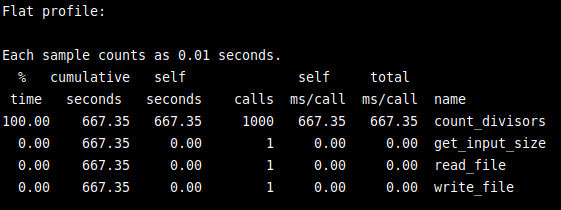
\includegraphics[width=1\textwidth]{Images/gprof.png}
    \vspace*{-0.5cm}
    \caption{Relatório gerado com a instância \emph{composite.txt}}
    \label{fig:map1}
\end{figure}

No entanto, sabemos que tal abordagem é inviável na prática com entradas cujo tamanho ultrapassa as centenas ou milhares de valores. Logo, foi decidido por paralelizar tal execução conforme o poder computacional à disposição. Todos os testes foram realizados em um computador com processador Intel© Core™ i7-8700, CPU que possui 6 núcleos e frequência de 3,20 GHz.

\subsection{Identificação das Oportunidades de Paralelização}

Como a maior parte do esforço computacional se concentra na execução da função que calcula o número de divisores de cada número, foi decidido por aplicar uma decomposição do domínio na implementação. Em outras palavras, a entrada é fragmentada em um número determinado de porções, estas que serão direcionadas para cada processo para execução em paralelo.

Como estratégia dominante na paralelização, optei por utilizar somente duas fases de comunicação durante toda a execução. Antes de qualquer processamento, o processo mestre (\(rank = 0\)) realiza a leitura do arquivo de entrada por completo para a memória e calcula os vetores correspondentes aos parâmetros reais de \emph{sendcount} e \emph{displacements} conforme o tamanho da entrada e o número de processos em execução. Tais vetores são de extrema relevância para a distribuição das porções para processamento paralelo.

Por fim, a aplicação de poucas fases de comunicação entre processos durante a execução do programa implicará em uma granularidade grossa para o processamento. Em outras palavras, a taxa de computação em relação a taxa de comunicação será grande. Após todos estes processos uma barreira (\emph{MPI\_Barrier}) é inserida para sincronizar todos os processos, sanando alguma dependência de computação, para então iniciar-se a cronometrar o tempo genuíno de computação com paralelismo. 

\subsection{Paralelização}

Nesta seção, é detalhado como o processo de paralelização do programa foi conduzido. Primeiramente, é apresentado como o paralelismo distribuído foi alcançado com auxílio das rotinas Open MPI, já inclusas na versão anterior deste programa. Após isto, focamos em como o paralelismo local em memória compartilhada foi obtido, utilizando OpenMP em uma abordagem híbrida.

\subsubsection{Open MPI}

A rotina selecionada para enviar os fragmentos do arquivo de entrada para cada processo escravo foi a \emph{MPI\_Scatterv}. O motivo por trás de tal escolha é de que uma de suas alternativas (\emph{MPI\_Scatter}) possui a restrição de que o tamanho da entrada deve ser divisível pelo número de processos. No caso da rotina \emph{MPI\_Scatterv}, essa restrição é inexistente, bastando fornecer os vetores correspondentes ao tamanho de cada porção e deslocamento, estes que foram calculados anteriormente conforme o tamanho da entrada.

Após a distribuição dos dados, cada processo fica responsável por um fragmento da entrada, estes que serão operados em paralelo com o uso da biblioteca OpenMP, calculando o número de divisores de cada valor sem que exista qualquer dependência entre tais que possa tornar o processo ocioso ou bloqueante.

Finalizada a computação paralelizada, os resultados do processamento de cada porção são agrupados utilizando a rotina complementar da \emph{MPI\_Scatterv}: a \emph{MPI\_Gatherv}. Novamente os vetores que correspondem ao tamanho de cada porção de cada processo e os deslocamentos são utilizados como parâmetros reais. Logo após é inserida uma nova barreira para sincronizar todos os processos, já que neste caso há grande probabilidade de que o tamanho dos fragmentos não sejam iguais entre si, encurtando ou atrasando o processamento. Por fim, a cronometragem é então finalizada para análise de resultados.

Concluídas todas estas etapas, o processo mestre então realiza a última operação de E/S, armazenando o número de divisores de cada valor do arquivo de entrada em sua respectiva ordem em um arquivo de saída.

\subsubsection{OpenMP}

Inicialmente, para implementar a paralelização em memória compartilhada utilizando OpenMP, pensou-se em alterar o cálculo do número divisores (\textit{divisors.c}) para testar múltiplas divisões em paralelo. No entanto, como o laço responsável por este cálculo possui uma instrução que pode interromper a execução do laço, tal implementação teve de ser remanejada.

Após a refatoração, o laço estava apto a ser paralelizado. No entanto, a retirada da condição que testava a divisão de um valor \(N\) até a sua raiz quadrada para identificar números primos foi removida. Isto significa que independentemente da entrada, seriam testadas divisões até um valor \(\frac{N}{2}\), o que tornava o tempo de execução entre todas as instâncias similar (desde que a magnitude dos mesmos também fosse próxima). 

Então, instâncias que executavam em um curto espaço de tempo (e.g., \textit{prime.txt}), agora estavam executando em um tempo similar às instâncias de pior caso (e.g., \textit{composite.txt}). As modificações realizadas na porção do código podem ser observadas na Figura \ref{fig:map2}. Como poderiam ocorrer condições de corrida com múltiplas \emph{threads} acessando a variável \textit{divisors}, foi adicionada uma cláusula \textit{reduction} para a mesma, impedindo possíveis inconsistências no cálculo do número de divisores.

\begin{figure}[H]
    \centering
    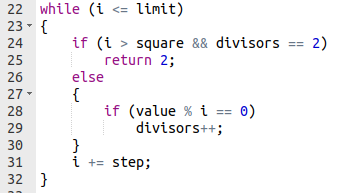
\includegraphics[width=.45\textwidth]{Images/old.png}
    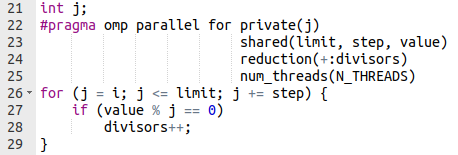
\includegraphics[width=.52\textwidth]{Images/new.png}
    \caption{Modificações para paralelizar o número de divisões}
    \label{fig:map2}
\end{figure}

Contudo, tal modificação foi revertida posteriormente para manter o desempenho observado anteriormente com diferentes tipos de instâncias. Para isto, o laço do programa principal foi modificado (\textit{parallel.c}). Desta forma, agora não são calculadas múltiplas divisões para cada valor, mas sim uma divisão para múltiplos valores de forma paralela. As modificações são apresentadas na Figura \ref{fig:map3}.

\begin{figure}[H]
    \centering
    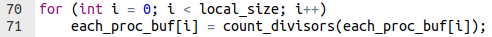
\includegraphics[width=.8\textwidth]{Images/p_before.png}
\end{figure}
\vspace*{-0.5cm}
\begin{figure}[H]
    \centering
    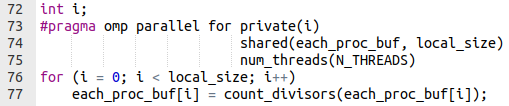
\includegraphics[width=.79\textwidth]{Images/p_after.png}
    \caption{Modificações para paralelizar o número de valores}
    \label{fig:map3}
\end{figure}

\section{Compilação e Execução}

\noindent Para compilar e executar o programa sequencialmente sem ou com perfilamento, basta executar os respectivos comandos via terminal:

\begin{center}
    \boxed{\textbf{\large{make sequential}}}\\
    \vspace{0.5cm}
    \boxed{\textbf{\large{make with\_prof}}}
\end{center}

\vspace{0.2cm}
\noindent Para executar a versão paralelizada do programa com OpenMP de forma (memória compartilhada), basta executar o seguinte comando via terminal:

\begin{center}
    \boxed{\textbf{\large{make shared\_omp}}}
\end{center}

\vspace{0.2cm}
\noindent Para executar a versão paralelizada do programa com Open MPI de forma compartilhada (localmente) ou distribuída (várias máquinas), basta executar os respectivos comandos via terminal:

\begin{center}
    \boxed{\textbf{\large{make shared\_mpi}}}\\
    \vspace{0.5cm}
    \boxed{\textbf{\large{make distributed\_mpi}}}
\end{center}

\vspace{0.2cm}
\noindent Para compilar e executar a versão com paralelismo híbrido do programa, basta executar o seguinte comando via terminal:

\begin{center}
    \boxed{\textbf{\large{make}}}\\
    \vspace{0.5cm}
    \boxed{\textbf{\large{make hybrid}}}
\end{center}

Os parâmetros de execução podem e devem ser alterados no arquivo \emph{Makefile} ou no arquivo \textbf{divisors.h}, alterando o arquivo de teste, número de processos, \emph{hostfile} e o número de \emph{threads}. Na compilação e execução, deve-se atentar para a explicitação do compilador MPI, utilizando opções distintas com ou sem caminhos relativos e absolutos como: \{mpicc, mpirun, home/\(<\)user\_name\(>\)/openmpi/bin/mpi\(<\)cc or run\(>\), \\home/\(<\)user\_name\(>\)/\(<\)user\_name\(>\)/openmpi/bin/mpi\(<\)cc or run\(>\)\}, sendo a última opção para uso em laboratório.

Também é possível gerar suas próprias instâncias de teste utilizando o \emph{script Python} presente no diretório \emph{instances}. Basta passar como parâmetros o tamanho máximo dos números em \emph{bits} e a quantidade a ser gerada executando o seguinte comando como exemplo:

\begin{center}
    \boxed{\textbf{\large{python3 instance\_generator.py -l 30 -n 10000}}}
\end{center}

\section{Análise de Resultados}

Como resultado mais relevante, podemos observar o comportamento completamente distinto do programa quanto ao tipo de entrada com a qual este está lidando. Não apenas sequencialmente, mas também em execução paralela, as instâncias que continham somente números primos foram as entradas com as quais o programa conseguiu executar com maior eficiência. Como mencionado na Subseção \ref{sub2}, todas as entradas possuem o mesmo tamanho, e os valores internos também possuem em média a mesma magnitude (até 30 \emph{bits}).

A razão pela qual o programa é mais eficiente com instâncias que contém maior quantidade de números primos, é de que o número de iterações no cálculo do número de divisores é reduzido drasticamente. Primeiramente, todo número primo é ímpar, logo o número de iterações no pior caso já é reduzido pela metade $\Bigl(\frac{N}{4}\Bigl)$. Além disso, o teste de primalidade reduz ainda mais a quantidade de iterações, ou seja, as divisões são testadas até o limite de \(\sqrt{N}\), com incremento de 2 no divisor a cada iteração. Como grande parte dos números presentes na entrada possuem grande quantidade de \emph{bits}, o número de iterações \(S\) é reduzido, tal que \(\sqrt{S} << \frac{N}{2}\).

Na Figura \ref{fig:map4}, podemos observar que o tempo de execução para instâncias com mil valores é completamente discrepante entre os tipos de entrada. Entradas contendo somente números primos são executadas em milissegundos, enquanto entradas contendo somente números compostos são executadas em minutos. Como é de se presumir, entradas que possuem uma mistura de tipos de números (primos e compostos) possuem como tempo de execução um "ponto médio" \hspace{0.1cm}entre os dois extremos (melhor caso e pior caso).

\vspace*{-0.5cm}
\begin{figure}[H]
    \centering
    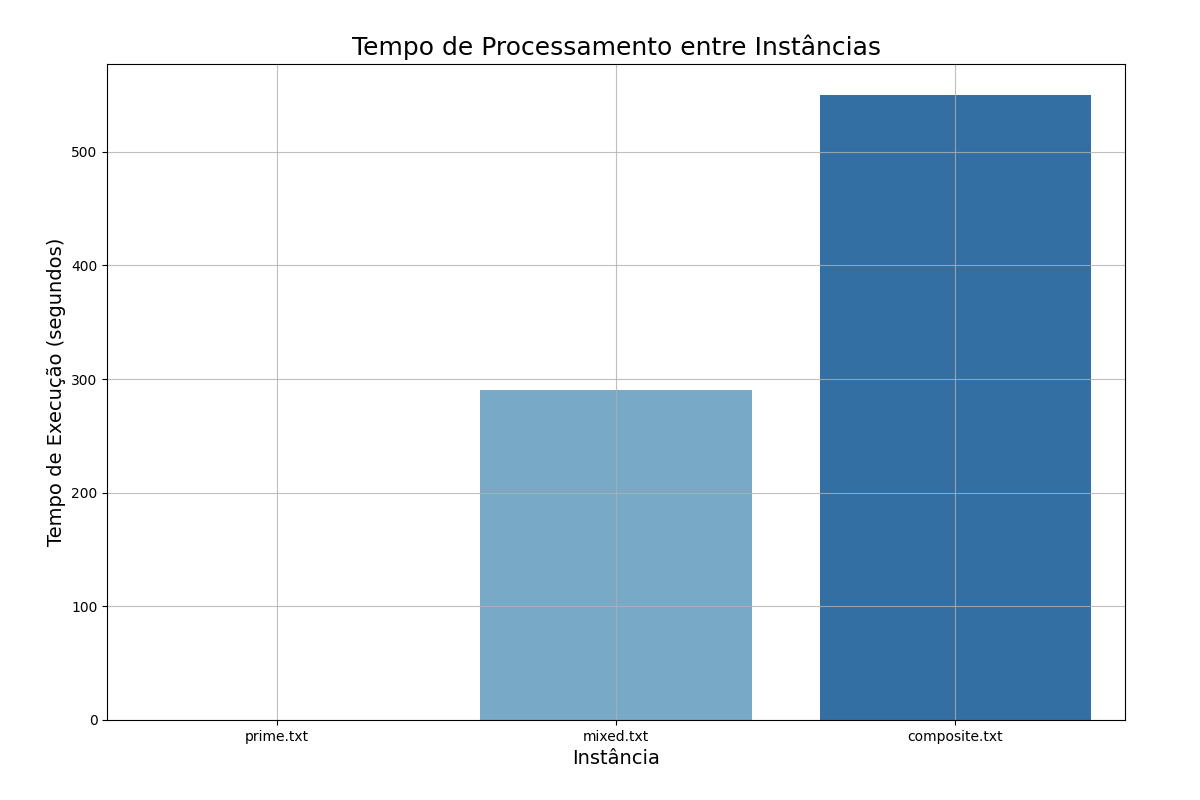
\includegraphics[width=1\textwidth]{Images/sequential.png}
    \vspace*{-1cm}
    \caption{Tempo de execução sequencial}
    \label{fig:map4}
\end{figure}

\subsection{Memória Compartilhada}

A partir deste ponto, será realizada uma comparação direta do desempenho do programa utilizando as bibliotecas em memória compartilhada e distribuída. Para fins de simplificação, foi selecionada uma única instância para execução dos testes. Tal instância corresponde à uma entrada de "caso médio" \hspace{0.1cm}(\emph{mixed.txt}) que possui tempos de execução razoáveis, ou seja, não são curtos como as entradas que só possuem números primos ou longos como as que só possuem números compostos. Isto auxilia na obtenção de resultados válidos, com boa interpretabilidade e relativamente rápidos de se obterem.

No escopo da memória compartilhada, o programa foi testado com 5 valores diferentes de parâmetro (\([2, 6]\)) para se mensurar os tempos de execução. Este parâmetro corresponde ao número de processos no caso de execução com Open MPI ou ao número de \emph{threads} na execução com OpenMP. Podemos observar na Figura \ref{fig:map5}, que o desempenho das bibliotecas na solução foi bastante similar, obtendo um \emph{speed up} de aproximadamente 4,7\(\times\) com OpenMP, e 4,9\(\times\) com Open MPI em relação ao tempo médio de execução sequencial.

\begin{figure}[H]
    \centering
    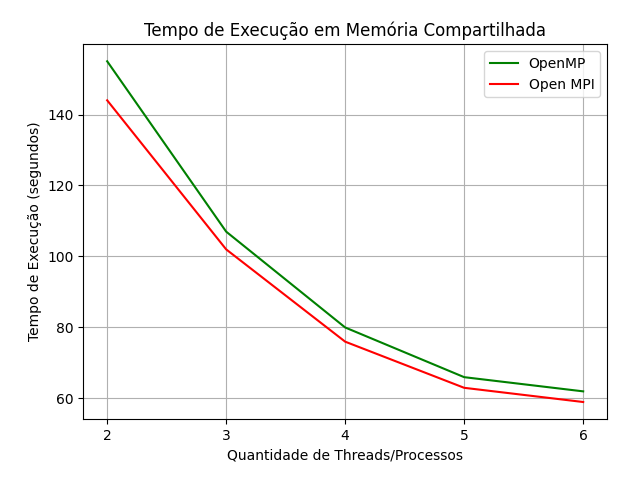
\includegraphics[width=1\textwidth]{Images/shared.png}
    \vspace*{-0.8cm}
    \caption{Tempos de execução com paralelismo em memória compartilhada}
    \label{fig:map5}
\end{figure}

\subsection{Memória Distribuída}

No escopo da memória distribuída, desta vez o parâmetro que sofreu variação foi a quantidade de máquinas envolvidas no processamento. É importante citar que todas as máquinas envolvidas nestes testes possuem o mesmo \emph{hardware}, e o número de \emph{threads} para execução em memória compartilhada local em cada máquina foi fixado em 6. Além disso, a máquina "mestre" \hspace{0.1cm}(\textit{rank = 0}) também processa parte da entrada no cálculo de divisores localmente.

Nos testes executados, constatou-se que quando se especifica 1 ou 2 processos MPI, a execução limita à utilização de 2 \emph{threads} por processo por padrão. Logo, não foi possível obter resultados válidos utilizando 2 processos (2 máquinas) e 6 \emph{threads}. No entanto, os restante dos resultados obtidos (Figura \ref{fig:map6}) são nítidos o suficiente para constatar que uma abordagem pura com Open MPI se sobressairá em termos de desempenho em relação à uma abordagem híbrida. Obteve-se um \emph{speed up} de aproximadamente 22\(\times\) com Open MPI em sua totalidade, e 20,5\(\times\) utilizando Open MPI em conjunto com OpenMP.

\begin{figure}[H]
    \centering
    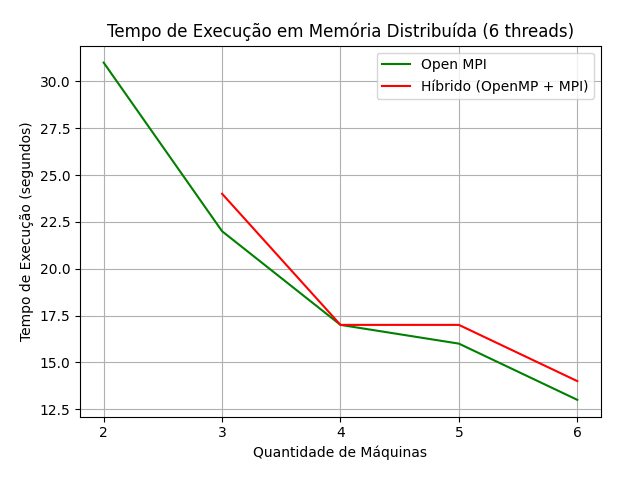
\includegraphics[width=1\textwidth]{Images/distributed.png}
    \vspace*{-0.8cm}
    \caption{Tempos de execução com paralelismo em memória distribuída}
    \label{fig:map6}
\end{figure}

\section{Limitações}

Como principal limitação, é possível citar o descumprimento parcial do modelo mestre-escravo. Na utilização da rotina \emph{MPI\_Scatterv}, os fragmentos do arquivo de entrada são particionados de forma que todos os processos envolvidos no comunicador recebem um fragmento (Figura \ref{fig:map7}). Em outras palavras, o processo mestre que deveria apenas ser responsável pelas operações de E/S (carregando o arquivo de entrada para a memória e armazenando o resultado em um arquivo de saída), também realiza o processamento do número de divisores de uma porção dos dados de entrada.

\begin{figure}[H]
    \centering
    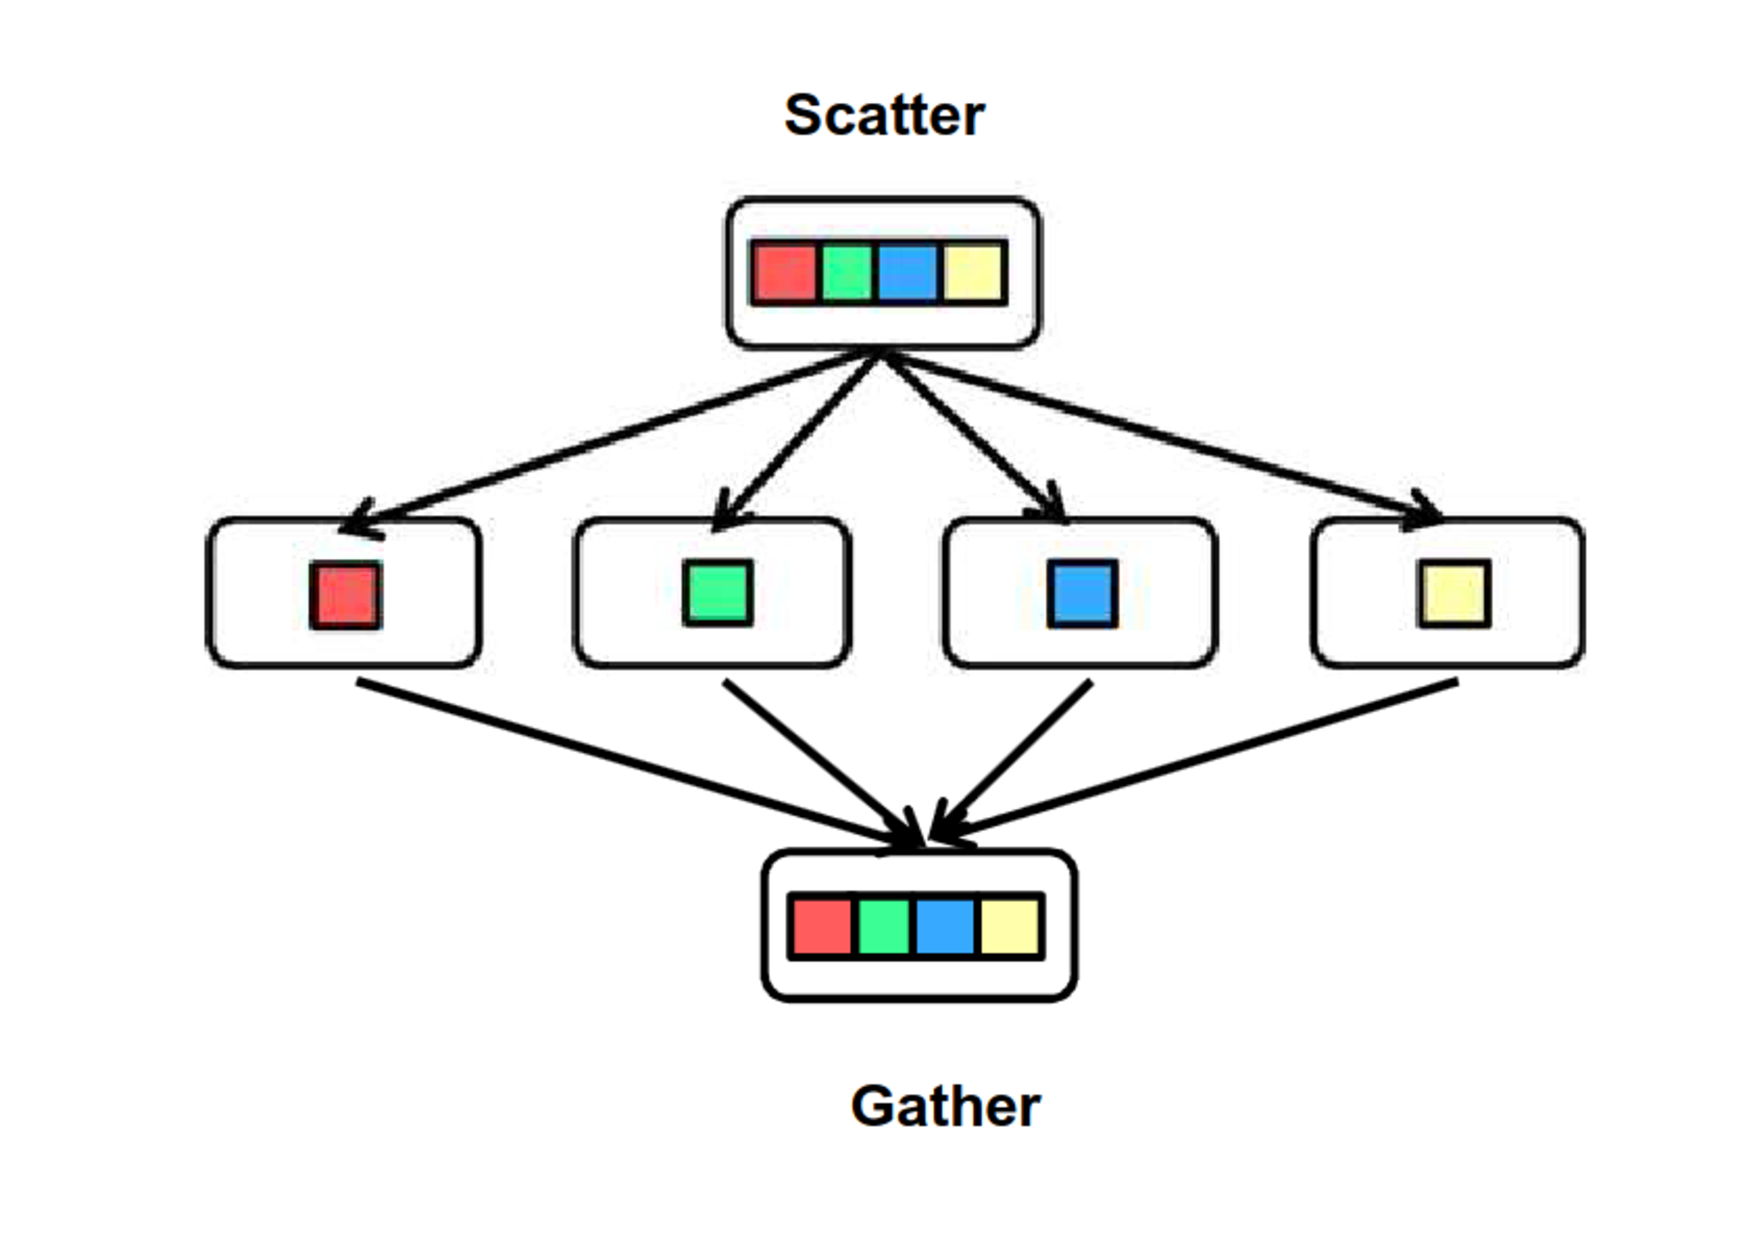
\includegraphics[width=0.85\textwidth]{Images/scatterv.pdf}
    \caption{Princípio de funcionamento das rotinas \emph{Scatter}}
    \vspace{0.2cm}
    \hspace*{15pt}\hbox{\small Fonte:\thinspace{\small \small{Mike Bailey, Oregon State University}\footnotemark}}\\
    \label{fig:map7}
\end{figure}

\footnotetext[9]{\scriptsize{Disponível em: \url{https://web.engr.oregonstate.edu/~mjb/cs575/Handouts/mpi.2pp.pdf}}}

Para contornar tal obstáculo, é possível criar um comunicador restrito aos processos escravos, para que então possa ser realizada a operação de \emph{Scatter} com o primeiro processo escravo como raiz (\(rank = 1\)), distribuindo os dados somente entre os processos escravos. Posteriormente o agrupamento dos dados seria realizado no comunicador global, para que então o processo mestre possa armazenar o resultado em um arquivo de saída.

\section{Trabalhos Futuros}

Como possíveis trabalhos futuros, pode ser interessante analisar o porquê a paralelização do programa produziu somente um \emph{speed up} sublinear, considerando que se trata de um problema embaraçosamente paralelo. Neste sentido, é uma opção analisar o \emph{overhead} proveniente da criação de \emph{threads}, processos e da comunicação entre os mesmo utilizando ambas bibliotecas.

Ainda em relação a \emph{overhead}, também seria interessante estudar o motivo pelo qual a abordagem híbrida obteve resultados inferiores à abordagem pura com Open MPI. Neste ponto, talvez possibilitasse identificar limitações de desempenho na preferência de uma biblioteca em detrimento de outra. 

Utilizando este trabalho como exemplo, embora a implementação da paralelização com OpenMP tenha se apresentado extremamente simples em relação ao manuseio com as rotinas Open MPI, o desempenho da abordagem híbrida no escopo de memória distribuída foi inferior.

\section{Conclusão}

Neste trabalho, foi explorada uma abordagem de computação paralela em memória distribuída e compartilhada utilizando uma abordagem híbrida com as bibliotecas Open MPI e OpenMP e para um problema bastante simples, mas no qual foi possível explorar diversos conceitos como decomposição de domínio, granularidade e paradigmas como mestre-escravo e SMPD (Single Program Multiple Data).

Com este exemplo didático, podemos observar de forma nítida, a complexidade por trás de se construir um programa que será executado em um conjunto de máquinas de forma indiscriminada e de forma híbrida, com uma biblioteca distinta responsável pelo paralelismo em memória compartilhada. Por isto, sempre é necessário ter extrema cautela no controle dos \emph{ranks} de cada processo, assim como seu número de \emph{threads} e a alocação e o acesso a memória realizado por cada parte do código.

\section*{Referências}

\begin{itemize}
    \item Hybrid MPI and OpenMP Parallel Programming: \url{https://www.openmp.org/wp-content/uploads/HybridPP_Slides.pdf};
    \item Parallel Programming with OpenMP: \url{https://web.njit.edu/~shahriar/class_home/HPC/omp3.pdf};
    \item OpenMP Programming: \url{https://www.cs.cmu.edu/afs/cs/academic/class/15418-s21/www/lectures/rec_04.pdf};
    \item The Message Passing Interface (MPI) - Parallelism on Distributed CPUs: \url{https://web.engr.oregonstate.edu/~mjb/cs575/Handouts/mpi.2pp.pdf};
    \item Profiling Programs With prof, gprof, and tcov: \url{https://docs.oracle.com/cd/E19059-01/stud.10/819-0493/OtherTools.html};
    \item MPI-size and number of OpenMP-Threads: \url{https://stackoverflow.com/questions/66262096/mpi-size-and-number-of-openmp-threads};
    \item How to use gettimeofday function in C language?: \url{https://linuxhint.com/gettimeofday_c_language/};
    \item scatter variable length data: \url{https://stackoverflow.com/questions/43642561/scatter-variable-length-data};
    \item Executing Shell Commands from a C program: \url{https://www.cs.uleth.ca/~holzmann/C/system/shell_commands.html};
    \item Material disponível no SIGAA na disciplina de Computação Paralela.
\end{itemize}

\end{document}